\section{Experiments} \label{exp}
%In this section, We first compare DIN with other methods including Wide\&Deep\cite{widedeep}, PNN\cite{PNN}, deepFM\cite{DeepFM} and Logistic Regression on two public dataset. DINs need to be evaluated on dataset with user behaviors, but not all dataset about CTR prediction contains user behaviors. Two public datasets with user behaviors: Amazon Dataset\footnote{http://jmcauley.ucsd.edu/data/amazon/} and MovieLens\footnote{https://grouplens.org/datasets/movielens/20m/} are used in this paper. Then our proposed methods are evaluated on Alibaba product data. We evaluate the effectiveness of the proposed structure of Deep Interest Network, activation function: Dice as well as the Mini-batch Aware Regularization Technique.

%In this section, we conduct empirical study on the performance of proposed DIN model and training techniques.
In this section, we present our experiments in detail, including datasets, evaluation metric, experimental setup, model comparison and the corresponding analysis.
Experiments on two public datasets with user behaviors as well as a dataset collected from the display advertising system in Alibaba demonstrate the effectiveness of proposed approach which outperforms state-of-the-art methods on the CTR prediction task.
Both the public datasets and experiment codes are made available\textsuperscript{\ref{code}}.%\footnote{Experiment codes on two public datasets are available at GitHub: https://github.com/zhougr1993/DeepInterestNetwork}.

\subsection{Datasets and Experimental Setup}
\textbf{Amazon Dataset\footnote{http://jmcauley.ucsd.edu/data/amazon/}.} 
Amazon Dataset contains product reviews and metadata from Amazon, which is used as benchmark dataset\cite{Amazon:AUC,AmazonData,ICCV_Amazon}. We conduct experiments on a subset named Electronics, which contains 192,403 users, 63,001 goods, 801 categories and 1,689,188 samples. User behaviors in this dataset are rich, with more than 5 reviews for each users and goods. Features include goods\_id, cate\_id, user reviewed goods\_id\_list and cate\_id\_list. Let all behaviors of a user be ($b_1, b_2, \ldots, b_k, \ldots, b_n$), the task is to predict the (k+1)-th reviewed goods by making use of the first k reviewed goods. 
    Training dataset is generated with $k = 1, 2, \ldots, n - 2$ for each user. In the test set, we predict the last one given the first $n-1$ reviewed goods. 
    For all models, we use SGD as the optimizer with exponential decay, in which learning rate starts at 1 and decay rate is set to 0.1. %We also tried Adam\cite{Adam}, which provides faster convergency but brings worse results than SGD for all deep models. 
    The mini-batch size is set to be $32$.

    
\textbf{MovieLens Dataset\footnote{https://grouplens.org/datasets/movielens/20m/}.} MovieLens data\cite{MovieLens} contains 138,493 users, 27,278 movies, 21 categories and 20,000,263 samples. To make it suitable for CTR prediction task, we transform it into a binary classification data. Original user rating of the movies is continuous value ranging from 0 to 5. We label the samples with rating of 4 and 5 to be positive and the rest to be negative. We segment the data into training and testing dataset based on userID. Among all 138,493 users, of which 100,000 are randomly selected into training set (about 14,470,000 samples) and the rest 38,493 into the test set (about 5,530,000 samples). The task is to predict whether user will rate a given movie to be above 3(positive label) based on historical behaviors. Features include movie\_id, movie\_cate\_id and user rated movie\_id\_list, movie\_cate\_id\_list. We use the same optimizer, learning rate and mini-batch size as described on Amazon Dataset.

\textbf{Alibaba Dataset.} We collected traffic logs from the online display advertising system in Alibaba, of which two weeks' samples are used for training and  samples of the following day for testing. The size of training and testing set is about 2 billions and 0.14 billion respectively. For all the deep models, the dimensionality of embedding vector is 12 for the whole 16 groups of features. %So the input dimension of first layer in MLP is 192. 
Layers of MLP is set by $192 \times 200 \times 80 \times 2$. Due to the huge size of data, we set the mini-batch size to be 5000 and use Adam\cite{Adam} as the optimizer. We apply exponential decay, in which learning rate starts at 0.001 and decay rate is set to 0.9.

The statistics of all the above datasets is shown in Table \ref{table:Statistics}. 
Volume of Alibaba Dataset is much larger than both Amazon and MovieLens, which brings more challenges. 

    
\begin{table}[]
%\setlength{\belowcaptionskip}{-1cm}
\caption{Statistics of datasets used in this paper.}
\small
\centering
\begin{threeparttable}
\begin{tabular}{lcccc}
\toprule
    Dataset       & Users & Goods\tnote{a} & Categories & Samples \\ \midrule
Amazon(Electro). & 192,403 & 63,001 & 801 & 1,689,188 \\ 
MovieLens. & 138,493 & 27,278 & 21 & 20,000,263 \\
Alibaba.  & 60 million & 0.6 billion & 100,000 & 2.14 billion \\ 
\bottomrule
\end{tabular}
\begin{tablenotes}%[para,flushleft]
        \item[a] For MovieLens dataset, goods refer to be movies.
        %\item[2] For security reasons we can only give an approximate number.
      \end{tablenotes}
      \end{threeparttable}
\label{table:Statistics}
\end{table}    




\begin{figure*}[!t]
\centering

\includegraphics[height=6.2in, width=6.2in, keepaspectratio]{images/exp/reg_new.png}
\caption{Performances of BaseModel with different regularizations on Alibaba Dataset. Training with fine-grained $goods\_ids$ features without regularization encounters serious overfitting after the first epoch. All the regularizations show improvement, among which our proposed mini-batch aware regularization performs best. Besides, well trained model with $goods\_ids$ features gets higher AUC than without them. It comes from the richer information that fine-grained features contained.}
\label{fig:adaptive_reg}
\end{figure*}






\subsection{Competitors}
\label{competitors}
\begin{itemize}
\item \textbf{LR\cite{ftrl}}. Logistic regression (LR) is a widely used shallow model before deep networks for CTR prediction task. We implement it as a weak baseline.       
\item \textbf{BaseModel}. As introduced in section\ref{sec:basemodel}, BaseModel follows the Embedding\&MLP architecture and is the base of most of subsequently developed deep networks for CTR modeling. It acts as a strong baseline for our model comparison.   
\item \textbf{Wide\&Deep\cite{widedeep}}. 
In real industrial applications, Wide\&Deep model has been widely accepted. 
It consists of two parts: i) wide model, which handles the manually designed cross product features, ii) deep model, which automatically extracts nonlinear relations among features and equals to the BaseModel. 
Wide\&Deep needs expertise feature engineering on the input of the "wide" module. 
We follow the practice in \cite{DeepFM} to take cross-product of user behaviors and candidates as wide inputs.
For example, in MovieLens dataset, it refers to the cross-product of user rated movies and candidate movies. 
\item \textbf{PNN\cite{PNN}.} PNN can be viewed as an improved version of BaseModel by introducing a product layer after embedding layer to capture high-order feature interactions. 
\item \textbf{DeepFM\cite{DeepFM}}. It imposes a factorization machines as "wide" module in Wide\&Deep saving feature engineering jobs. 
\end{itemize}
\subsection{Metrics}
\label{metric}
In CTR prediction field, AUC is a widely used metric\cite{fawcett:roc}. 
It measures the goodness of order by ranking all the ads with predicted CTR, including intra-user and inter-user orders. 
An variation of user weighted AUC is introduced in \cite{Amazon:AUC,zhu2017optimized} which measures the goodness of intra-user order by averaging AUC over users and is shown to be more relevant to online performance in display advertising system. 
We adapt this metric in our experiments. For simplicity, we still refer it as AUC. 
It is calculated as follows:
\begin{small}
\begin{equation} \label{imps-guac}
\text{AUC} = \frac{\sum_{i=1}^{n} \#impression_i \times \text{AUC}_{i}}{\sum_{i=1}^{n} \#impression_i},
\end{equation}
\end{small}
where $n$ is the number of users, $\#impression_i$ and $\text{AUC}_i$ are the number of impressions and AUC corresponding to the $i$-th user. 

Besides, we follow \cite{yan2014coupled} to introduce RelaImpr metric to measure relative improvement over models. For a random guesser, the value of AUC is $0.5$. Hence RelaImpr is defined as below: 
\begin{small}
\begin{equation}
RelaImpr = \left(\frac{\text{AUC(measured model)} -0.5}{\text{AUC(base model)} - 0.5} - 1\right) \times 100\%.
\end{equation}
\end{small}



\begin{table}[]
%\setlength{\belowcaptionskip}{-1cm}
\caption{Model Coparison on Amazon Dataset and MovieLens Dataset. All the lines calculate RelaImpr by comparing with BaseModel on each dataset respectively.}
\centering
\begin{threeparttable}
\begin{tabular}{lcccc}
\toprule
\multirow{2}{*}{Model}  & \multicolumn{2}{c}{MovieLens.} & \multicolumn{2}{c}{Amazon(Electro).}  \\ 
& AUC & RelaImpr & AUC & RelaImpr \\ \midrule
LR  & 0.7263 & -1.61\% & 0.7742 & -24.34\%  \\
BaseModel & 0.7300 & 0.00\% & 0.8624 & 0.00\%  \\
Wide\&Deep & 0.7304 & 0.17\% & 0.8637 & 0.36\%  \\
PNN  & 0.7321 & 0.91\% & 0.8679 & 1.52\%  \\
DeepFM  & 0.7324 & 1.04\% & 0.8683 & 1.63\% \\
\textbf{DIN} & \textbf{0.7337} & \textbf{1.61\%} & \textbf{0.8818} & \textbf{5.35}\%\\
\textbf{DIN with Dice}\tnote{a} & \textbf{0.7348} & \textbf{2.09\%} & \textbf{0.8871} & \textbf{6.82\%} \\ \bottomrule
\end{tabular}
\begin{tablenotes}%[para,flushleft]
        \item[a] Other lines except LR use PReLU as activation function.
      \end{tablenotes}
      \end{threeparttable}
\label{table:exptablePublic}
\end{table}
\vspace*{-0.4cm}





\subsection{Result from model comparison on Amazon Dataset and MovieLens Dataset}
Table \ref{table:exptablePublic} shows the results on Amazon dataset and MovieLens dataset.
%All the experiments are repeated 5 times with different seed, and the influence of random initialization on AUC is less than 0.0002.
All experiments are repeated 5 times and averaged results are reported. The influence of random initialization on AUC is less than 0.0002.
Obviously, all the deep networks beat LR model significantly, which indeed demonstrates the power of deep learning.   
PNN and DeepFM with specially designed structures preform better than Wide\&Deep. 
DIN performs best among all the competitors. 
Especially on Amazon Dataset with rich user behaviors, DIN stands out significantly.
We owe this to the design of local activation unit structure in DIN.
DIN pays attentions to the locally related user interests by soft-searching for parts of user behaviors that are relevant to candidate ad. With this mechanism, DIN obtains an adaptively varying representation of user interests, greatly improving the expressive ability of model compared with other deep networks.  
Besides, DIN with Dice brings further improvement over DIN, which verifies the effectiveness of the proposed data adaptive activation function Dice.  




\begin{table}[]
%\setlength{\belowcaptionskip}{-1cm}
\caption{Best AUCs of BaseModel with different regularizations on Alibaba Dataset corresponding to Fig.\ref{fig:adaptive_reg}. All the other lines calculate RelaImpr by comparing with first line.}
\small
\centering
\begin{threeparttable}
\begin{tabular}{p{5cm} p{0.6cm}<{\centering} p{0.8cm}<{\centering}}
\toprule
 Regularization    & AUC  &RelaImpr \\ \midrule
Without goods\_ids feature and Reg. & 0.5940 & 0.00\% \\
With goods\_ids feature without Reg. & 0.5959  & 2.02\% \\
With goods\_ids feature and Dropout Reg. & 0.5970  & 3.19\%  \\
With goods\_ids feature and Filter Reg.  & 0.5983& 4.57\%  \\
With goods\_ids feature and Difacto Reg.  & 0.5954 & 1.49\%  \\
\textbf{With goods\_ids feature and MBA. Reg.}  & \textbf{0.6031}  & \textbf{9.68\%}  \\ \bottomrule
\end{tabular}
\end{threeparttable}
\label{table:expreg}
\end{table}



\subsection{Performance of regularization}
\label{sec:reg}
As the dimension of features in both Amazon Dataset and MovieLens Dataset is not high (about 0.1 million), 
all the deep models including our proposed DIN do not meet grave problem of overfitting.
However, when it comes to the Alibaba dataset from the online advertising system which contains higher dimensional sparse features, overfitting turns to be a big challenge. 
For example, when training deep models with fine-grained features (e.g., features of $goods\_ids$ with dimension of 0.6 billion in Table \ref{table_feature_set}), serious overfitting occurs after the first epoch without any regularization, which causes the model performance to drop rapidly, as the dark green line shown in Fig.\ref{fig:adaptive_reg}.     
For this reason, we conduct careful experiments to check the performance of several commonly used regularizations.
%Here we compare several commonly used regularizations.
\begin{itemize}
\item \textbf{Dropout\cite{dropout}}. Randomly discard $50\%$ of feature ids in each sample.
\item \textbf{Filter}. Filter visited $goods\_id$ by occurrence frequency in samples and leave only the most frequent ones. In our setting, top $20$ million $goods\_ids$ are left.
\item \textbf{Regularization in DiFacto\cite{difacto}}. Parameters associated with frequent features are less over-regularized.
\item \textbf{MBA}. Our proposed \textbf{M}ini-\textbf{B}atch \textbf{A}ware regularization method (Eq.\ref{eq:batch}). Regularization parameter $\lambda$ for both DiFacto and MBA is searched and set to be $0.01$.
\end{itemize}



Fig.\ref{fig:adaptive_reg} and Table \ref{table:expreg} give the comparison results. 
Focusing on the detail of Fig.\ref{fig:adaptive_reg}, model trained with fine-grained $goods\_ids$ features brings large improvement on the test AUC performance in the first epoch, compared without it. 
However, overfitting occurs rapidly in the case of training without regularization (dark green line).   
Dropout prevents quick overfitting but causes slower convergence. 
Frequency filter relieves overfitting to a degree.
Regularization in DiFacto sets a greater penalty on $goods\_id$ with high frequency, which performs worse than frequency filter.
Our proposed mini-batch aware(MBA) regularization performs best compared with all the other methods, which prevents overfitting significantly. 

Besides, well trained models with $goods\_ids$ features show better AUC performance than without them. This is duo to the richer information that fine-grained features contained.
Considering this, although frequency filter performs slightly better than dropout, it throws away most of low frequent ids and may lose room for models to make better use of fine-grained features. 


\subsection{Result from model comparison on Alibaba Dataset}
Table \ref{table:ali} shows the experimental results on Alibaba dataset with full feature sets as shown in Table \ref{table_feature_set}.
As expected, LR is proven to be much weaker than deep models. 
Making comparisons among deep models, we report several conclusions.  
First, under the same activation function and regularization, DIN itself has achieved superior performance compared with all the other deep networks including BaseModel, Wide\&Deep, PNN and DeepFM. DIN achieves 0.0059 absolute AUC gain and $6.08\%$ RelaImpr over BaseModel. It validates again the useful design of local activation unit structure.   
Second, ablation study based on DIN demonstrates the effectiveness of our proposed training techniques. Training DIN with mini-batch aware regularizer brings additional 0.0031 absolute AUC gain over dropout. Besides, DIN with Dice brings additional 0.0015 absolute AUC gain over PReLU. 
%In all, training DIN with the two proposed techniques together brings total 0.0054 AUC gain. 

Taken together, DIN with MBA regularization and Dice achieves total $11.65\%$ RelaImpr and 0.0113 absolute AUC gain over BaseModel. Even compared with competitor DeepFM which performs best on this dataset, DIN still achieves 0.009  absolute AUC gain. 
It is notable that in commercial advertising systems with hundreds of millions of traffics, 0.001 absolute AUC gain is significant and worthy of model deployment empirically. 
DIN shows great superiority to better understand and make use of the characteristics of user behavior data. 
Besides, the two proposed techniques further improve model performance and provide powerful help for training large scale industrial deep networks.   

\begin{table}[]
%\setlength{\belowcaptionskip}{-0.5cm}
\caption{Model Comparison on Alibaba Dataset with full feature sets. All the lines calculate RelaImpr by comparing with BaseModel. 
DIN significantly outperforms all the other competitors. Besides, training DIN with our proposed mini-batch aware regularizer and Dice activation function brings further improvements.}
\small
\centering
\begin{threeparttable}
\begin{tabular}{p{4cm} p{1.5cm}<{\centering} p{1.5cm}<{\centering}}
\toprule
Model & AUC & RelaImpr \\ \midrule
LR                                  & 0.5738 &  - 23.92\%  \\    
BaseModel\tnote{a,b}               & 0.5970 &  0.00\% \\
Wide\&Deep\tnote{a,b}               & 0.5977 &  0.72\%  \\
PNN\tnote{a,b}                      & 0.5983 &  1.34\%  \\
DeepFM\tnote{a,b}                   & 0.5993 &  2.37\%  \\
\textbf{DIN Model\tnote{a,b}}       & \textbf{0.6029} & \textbf{6.08\%} \\
\textbf{DIN with MBA Reg.\tnote{a}} & \textbf{0.6060} &  \textbf{9.28}\%  \\
\textbf{DIN with Dice \tnote{b}}    & \textbf{0.6044} &  \textbf{7.63}\%  \\
\textbf{DIN with MBA Reg. and Dice} & \textbf{0.6083} &  \textbf{11.65\%}  \\ \bottomrule
\end{tabular}
\begin{tablenotes}%[para,flushleft]
        \item[a] These lines are trained with PReLU as the activation function. 
        \item[b] These lines are trained with dropout regularization. 
      \end{tablenotes}
      \end{threeparttable}
\label{table:ali}
\end{table}


\subsection{Result from online A/B testing}
Careful online A/B testing in the display advertising system in Alibaba was conducted from 2017-05 to 2017-06. 
During almost a month's testing,  DIN trained with the proposed regularizer and activation function contributes up to 10.0\% CTR and 3.8\% RPM(Revenue Per Mille) promotion\footnote{In our real advertising system, ads are ranked by $\textsl{CTR}^\alpha \cdot \textsl{bid-price}$ with $\alpha > 1.0$, which controls the balance of promotion of CTR and RPM.} compared with the introduced BaseModel, the last version of our online-serving model. This is a significant improvement and demonstrates the effectiveness of our proposed approaches. Now DIN has been deployed online and serves the main traffic.  

It is worth mentioning that online serving of industrial deep networks is not an easy job with hundreds of millions of users visiting our system everyday. Even worse, at traffic peak our system serves more than 1 million users per second. It is required to make realtime CTR predictions with high throughput and low latency. For example, in our real system we need to predict hundreds of ads for each visitor in less than 10 milliseconds.  
In our practice, several important techniques are deployed for accelerating online serving of industrial deep networks under the CPU-GPU architecture:  
i) \textsl{request batching} which merges adjacent requests from CPU to take advantage of GPU power,
ii) \textsl{GPU memory optimization} which improves the access pattern to reduce wasted transactions in GPU memory,
iii) \textsl{concurrent kernel computation} which allows execution of matrix computations to be processed with multiple CUDA kernels concurrently.           
In all, optimization of these techniques doubles the QPS (Query Per Second) capacity of a single machine practically. 
Online serving of DIN also benefits from this. 


\subsection{Visualization of DIN}
\label{visual_din}
Finally we conduct case study to reveal the inner structure of DIN on Alibaba dataset.
%DIN designs the activation unit to locally activate the related behaviors with respect to candidate ads. 
We first examine the effectiveness of local activation unit. 
Fig.\ref{fig:att_case} illustrates the activation intensity of user behaviors with respect to a candidate ad.
As expected, behaviors with high relevance to candidate ad are weighted high.


%\begin{figure*}[!h]
\begin{figure}[!h]
\centering
%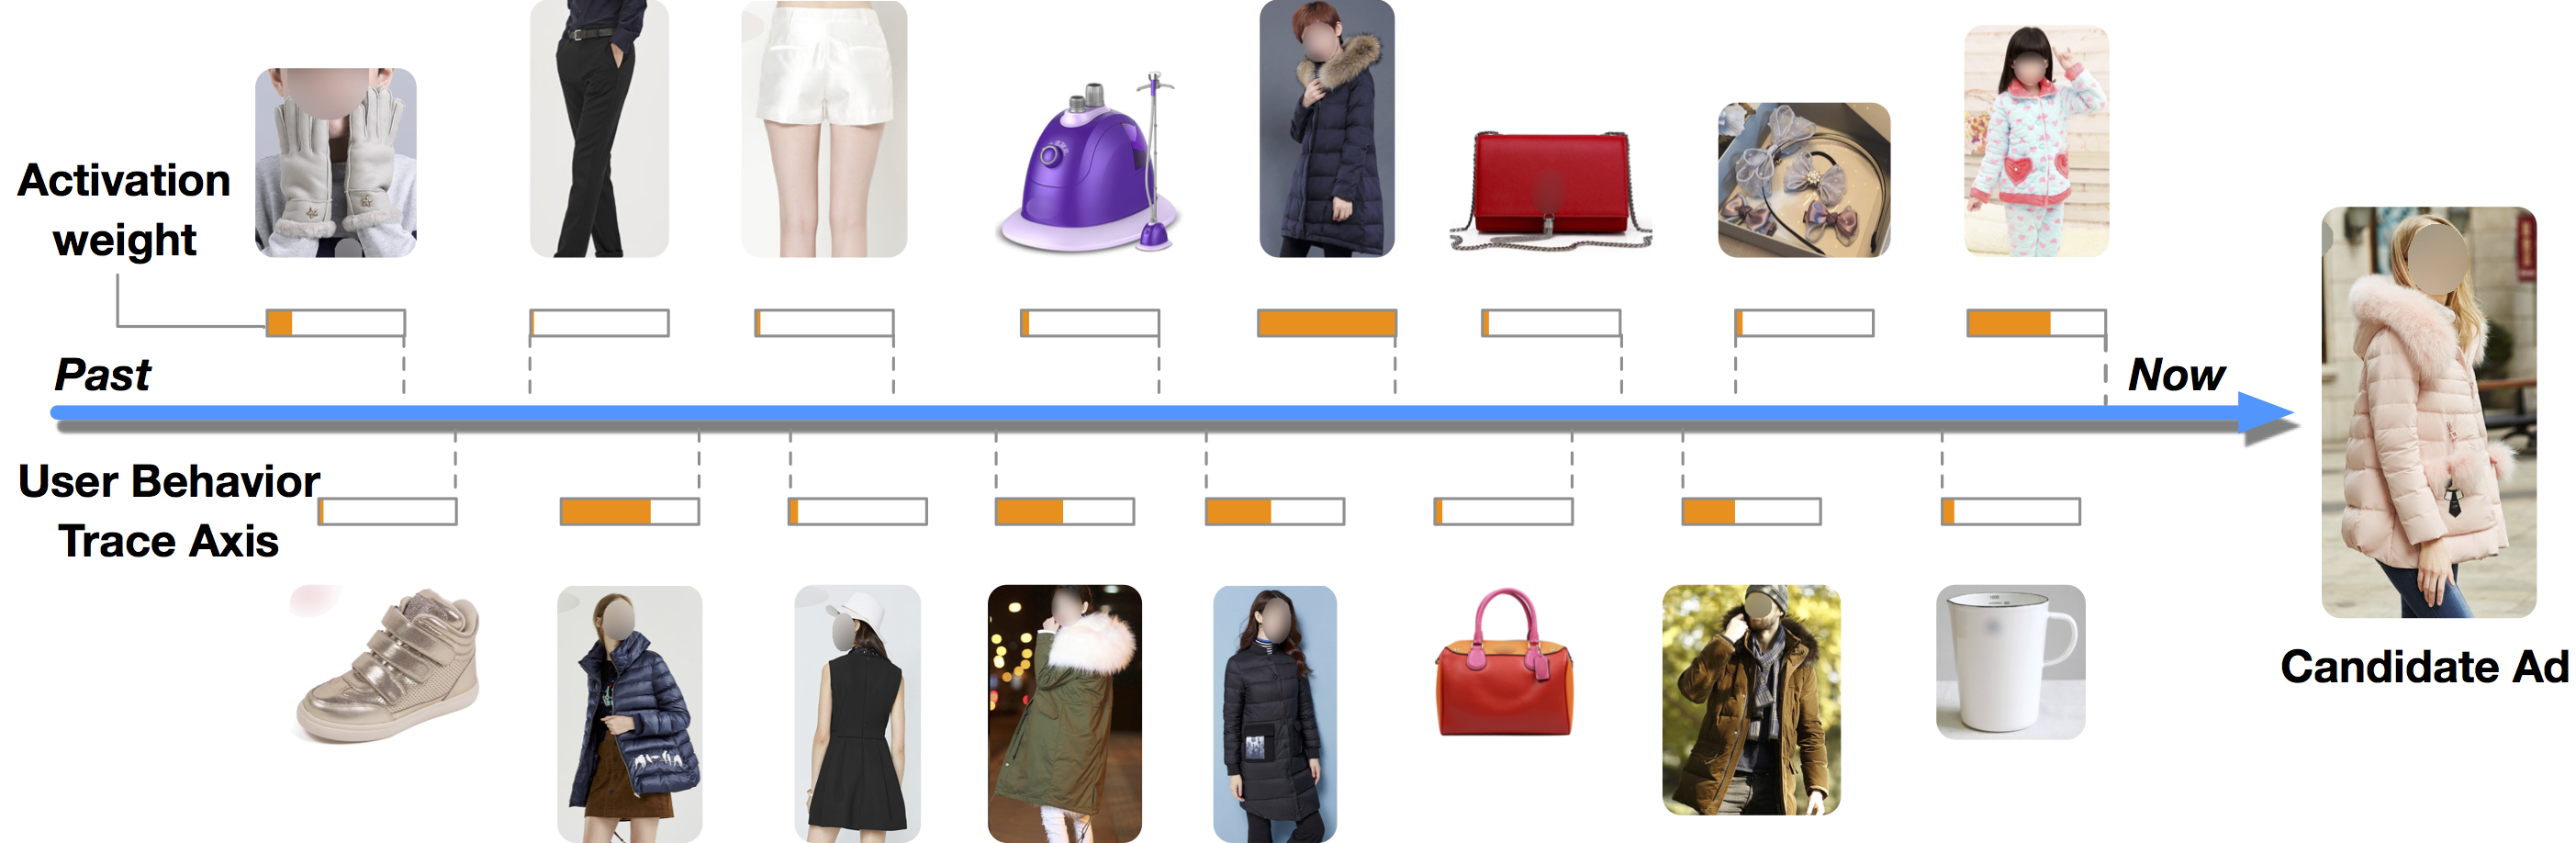
\includegraphics[height=3.5in, width=5in, keepaspectratio]{images/omni/attention_timeline_fix.pdf}
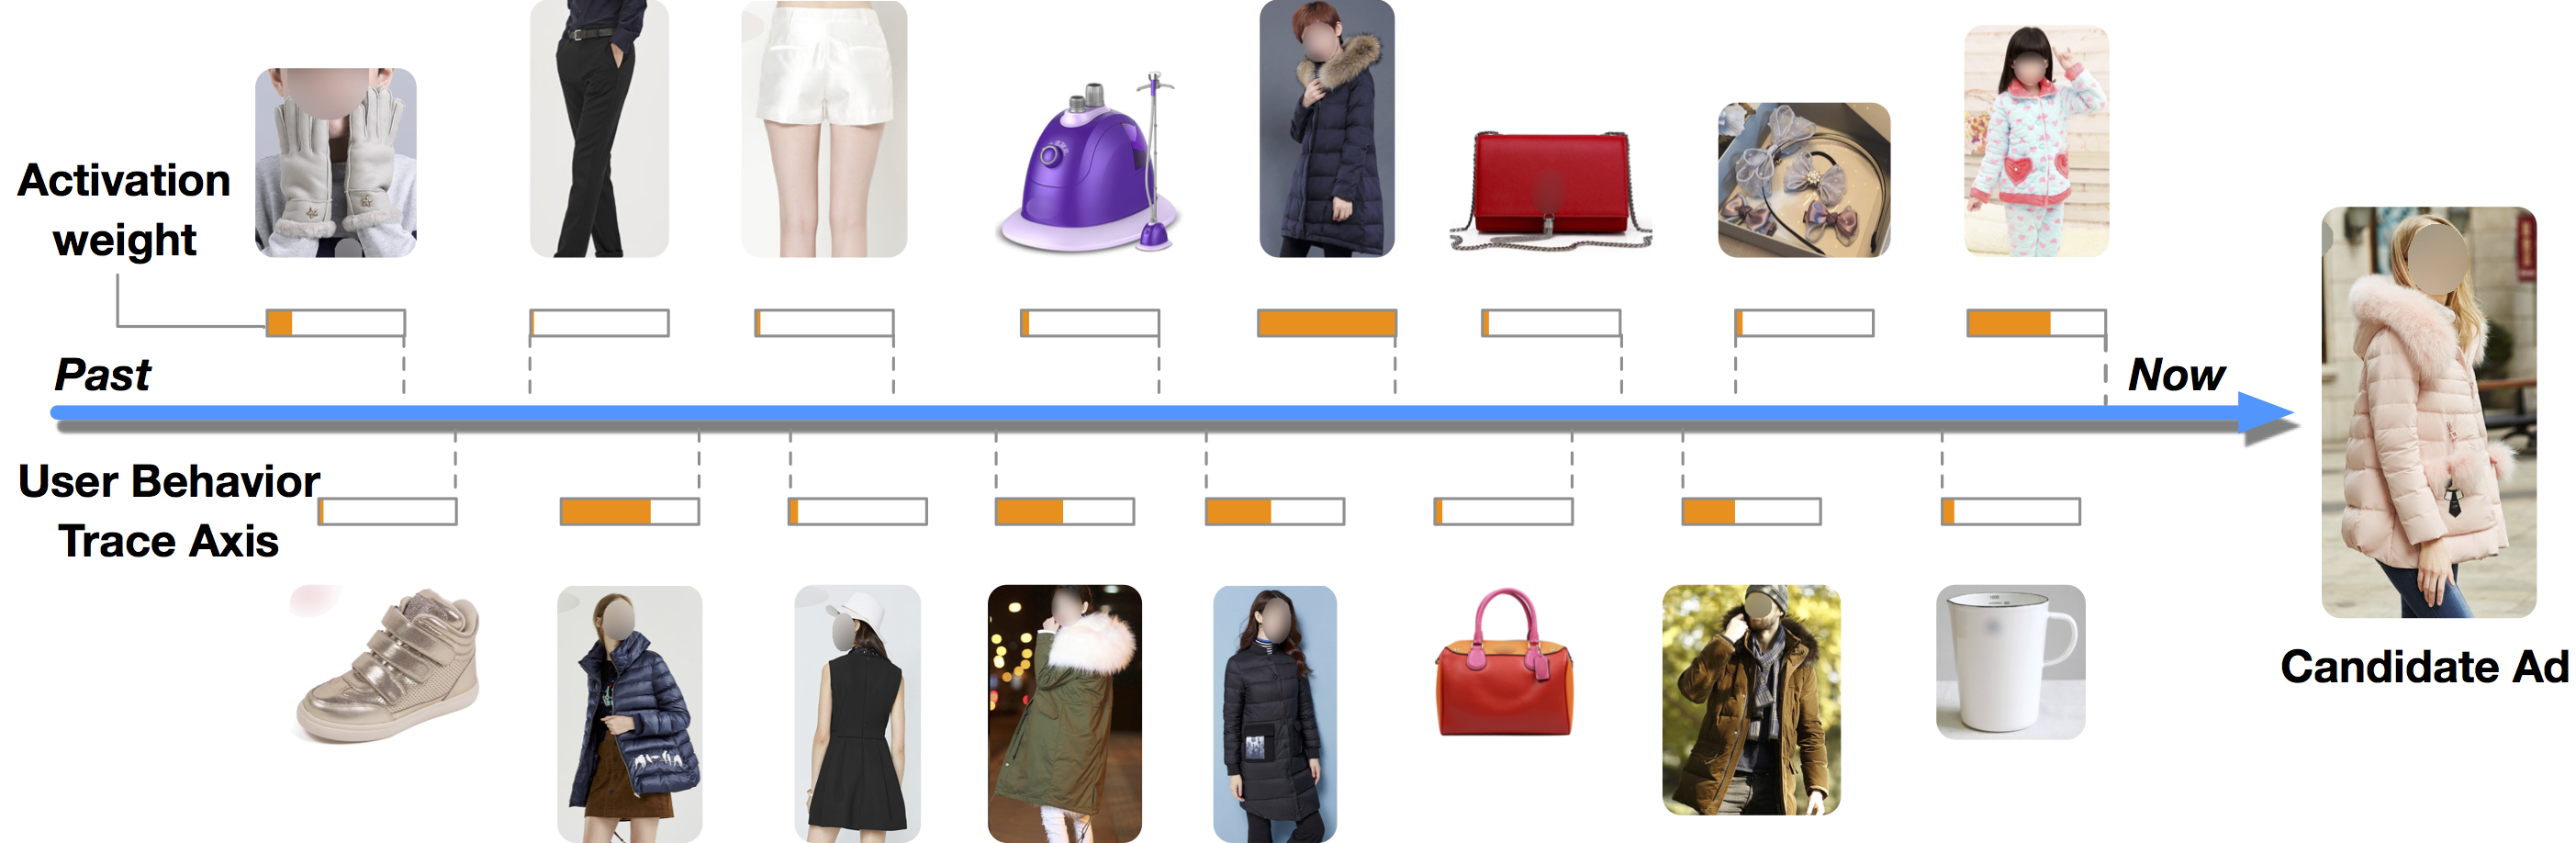
\includegraphics[height=2.5in, width=3.5in, keepaspectratio]{images/omni/attention_timeline_fix.png}
\caption{Illustration of adaptive activation in DIN. Behaviors with high relevance to candidate ad get high activation weight. }
\label{fig:att_case}
%\end{figure*}
\end{figure}


We then visualize the learned embedding vectors.
Taking the young mother mentioned before as example, we randomly select 9 categories (dress, sport shoes, bags, etc) and 100 goods of each category as the candidate ads for her.
Fig.\ref{fig:TDdiagram} shows the visualization of embedding vectors of goods with t-SNE\cite{tsne} learned by DIN, in which points with same shape correspond to the same category. 
We can see that goods with same category almost belong to one cluster, which shows the clustering property of DIN embeddings clearly.
Besides, we color the points that represent candidate ads by the prediction value. Fig.\ref{fig:TDdiagram} is also a heat map of this mother's interest density distribution for potential  candidates in embedding space. It shows DIN can form a multimodal interest density distribution in candidates' embedding space for a certain user to capture his/her diverse interests. 




\begin{figure}[!t]
%\setlength{\belowcaptionskip}{-0.5cm}
\centering
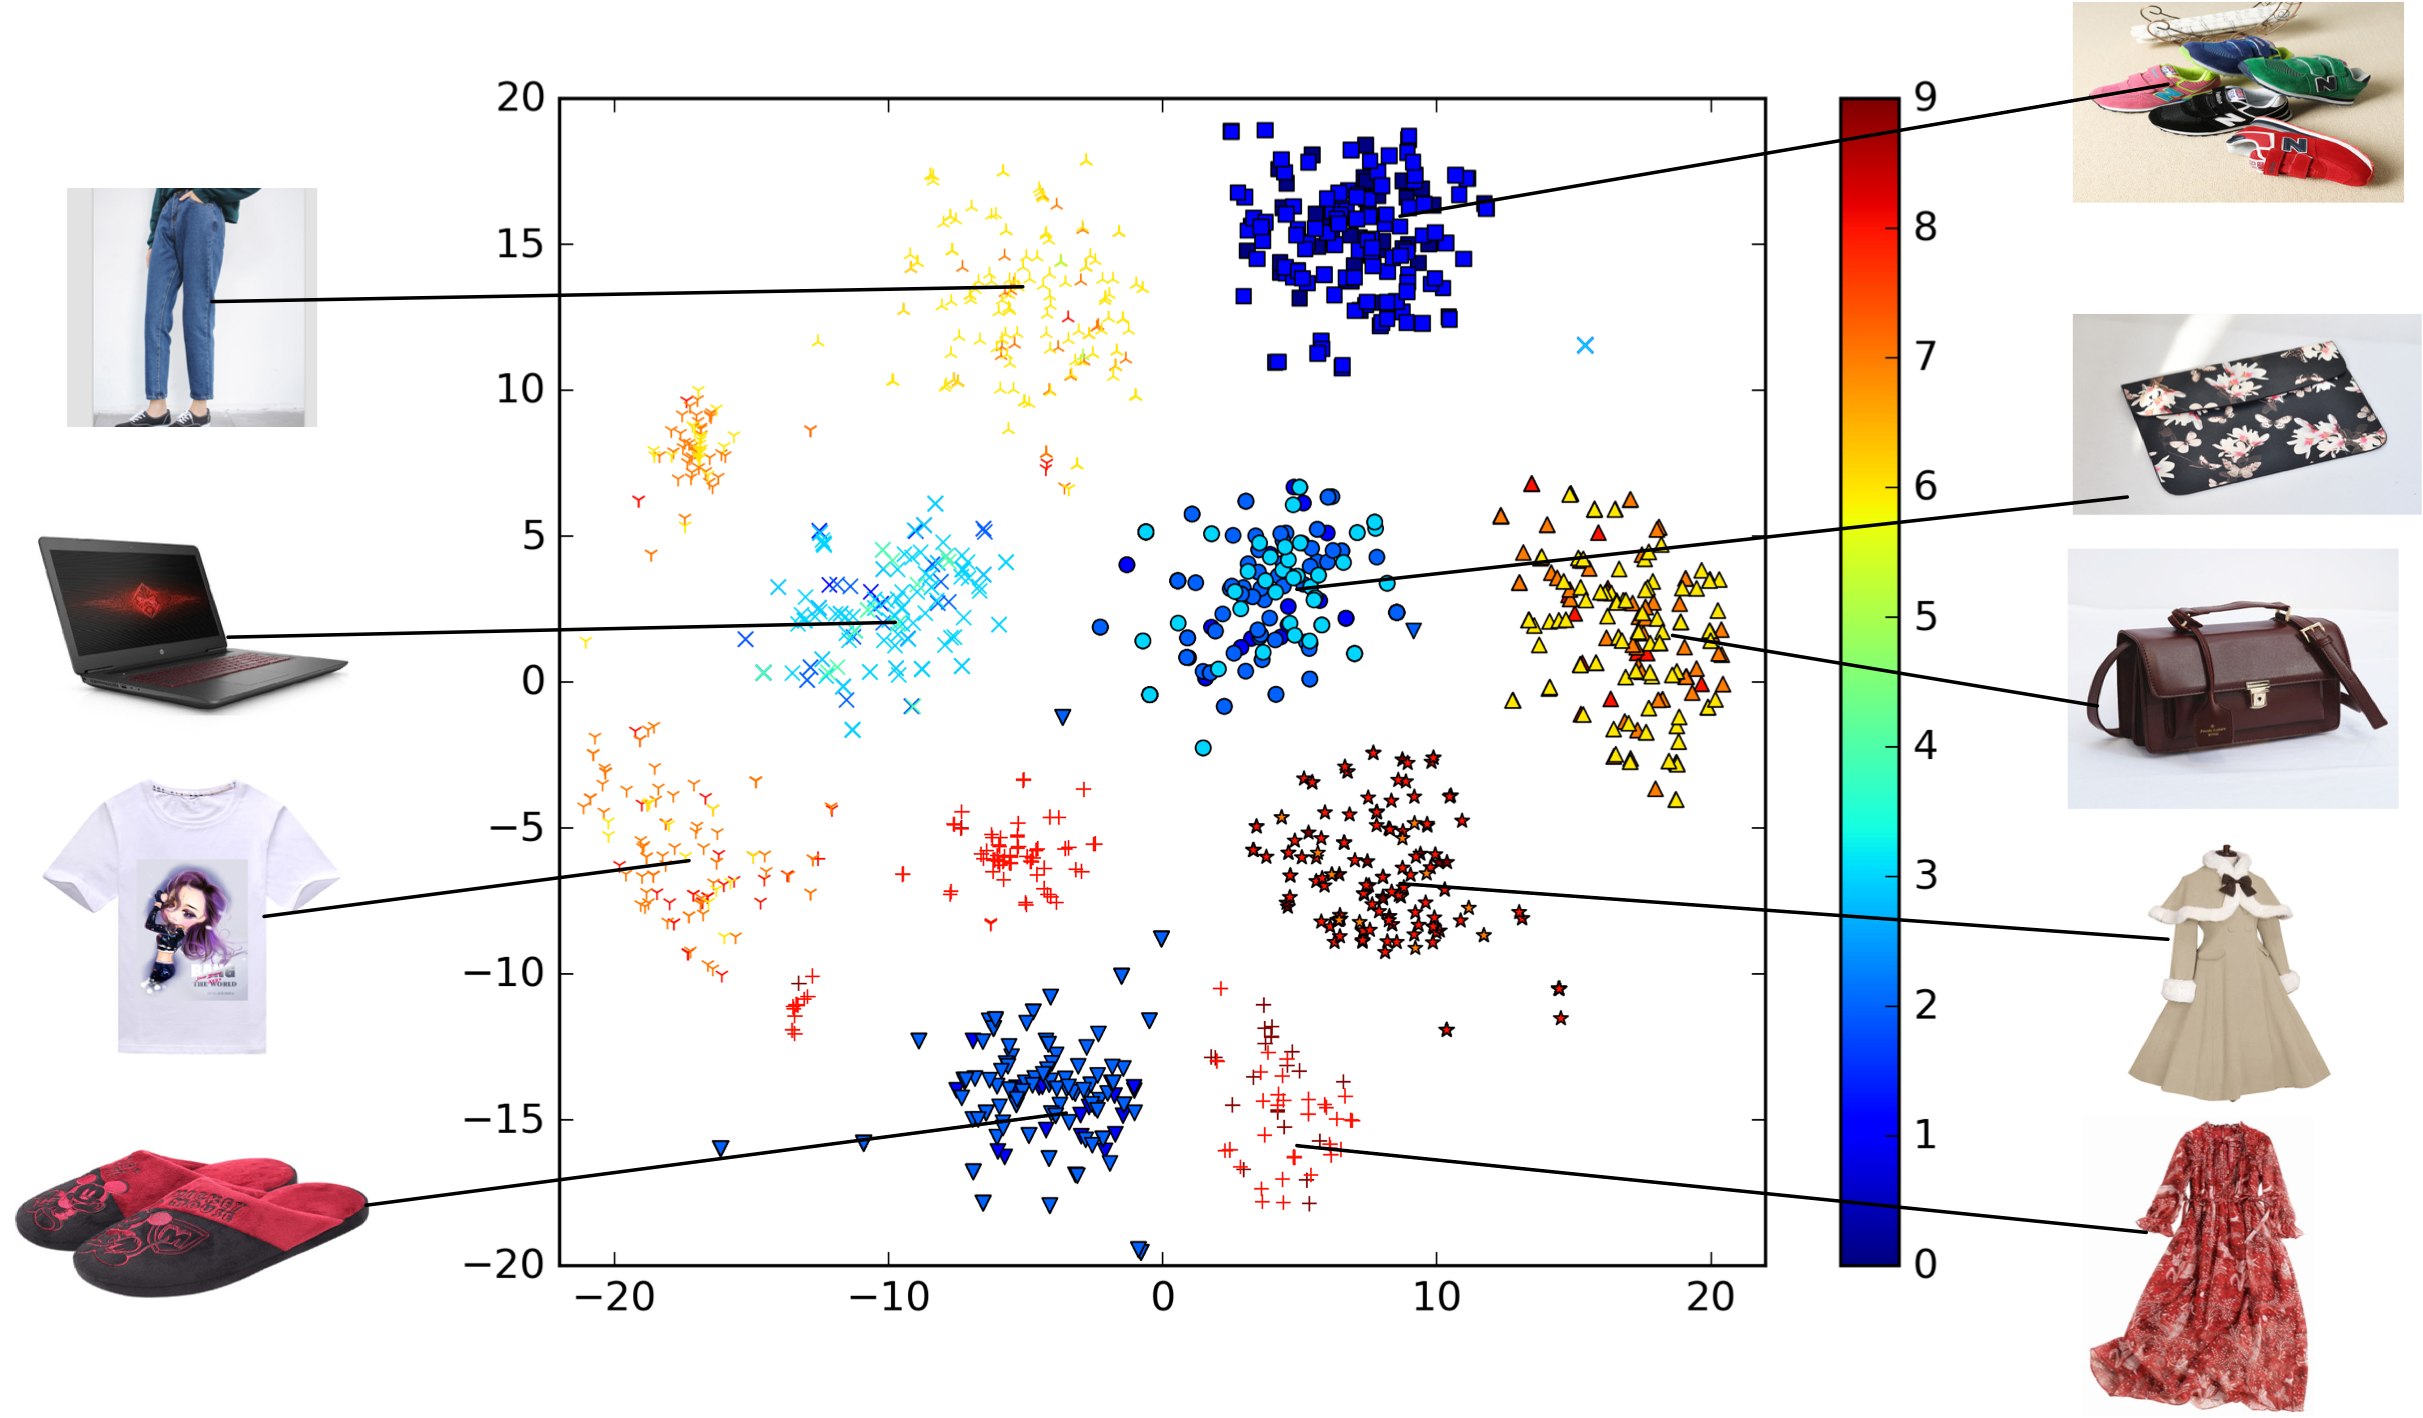
\includegraphics[height=2.5in, width=3.5in, keepaspectratio]{images/omni/TDdiagram.png}
\caption{Visualization of embeddings of goods in DIN. Shape of points represents category of goods. Color of points corresponds to CTR prediction value.}
\label{fig:TDdiagram}
\end{figure}



%Besides, we color the points that represent candidate ads by the prediction value. 
%Hot(red) points get higher CTR than cold(blue) ones.
%The red points appear in more than one clusters.
%Different categories of goods appearing the her historical behaviors are colored hot(red), which get higher CTR than those random candidates with cold(blue) color.  
%This demonstrates that DIN is able to capture diverse interests of a certain user, by forming a multimodal probability distribution of user interests in the embedding space.




